\section{コサイン類似度を用いたi-vectorの性質の調査}
\label{section:pre_cos}
本調査では、発話の長さによって同一話者の発話間の場合と異なる話者の発話間の2つの場合でi-vectorのコサイン類似度がとる値についての調査を行う。

\subsection{使用する音声データ}
\label{section:detail_ATR}
UBMモデルの学習データおよびコサイン類似度を用いたi-vectorの性質の調査に読み上げ音声\cite{ATR}を使用した。読み上げ音声には、男女各110人$×$50発話分が収録されている。

\subsection{調査方法}
各話者の音声データから一発話を取り出し、それ以外の音声データとのi-vectorのコサイン類似度を算出する。また、同一話者の発話間の場合と異なる話者の発話間の2つの場合で発話の長さごとのコサイン類似度が取る値の平均の検証を行う。\par

\subsection{コサイン類似度の算出条件}
i-vectorの抽出には、ALIZEとLIR RAL\cite{alize}を用いる。読み上げ音声に収録されている各発話データからi-vectorを抽出する。発話データから抽出する音響特徴パラメータを表\ref{iv_feature}に示す。また混合数は32とした。

\begin{table}[H]
  \begin{center}
    \caption{使用する音響特徴パラメータ}
    \label{iv_feature}
    \begin{tabular}{|c||c|} \hline
      特徴量 & 次元数\\ \hline
      MFCC & 19  \\ 
      POW & 1  \\ 
      $\Delta$MFCC & 19 \\ 
      $\Delta$POW & 1 \\ 
      $\Delta\Delta$MFCC & 19 \\ 
      $\Delta\Delta$POW & 1 \\ \hline
      計 & 60 \\ \hline
    \end{tabular}
  \end{center}
\end{table}

本稿では、音響特徴量のひとつとしてメル周波数ケプストラム係数(MFCC)を用いる。メル周波数ケプストラム係数(Mel - Frequency Cepstrum Coefficient : MFCC)とは、メル周波数という人間の音の高低に対する感覚尺度を考慮した特徴量であり、音声スペクトルから係数スペクトルを抽出したものである。これは一般的に、音声の特徴を抽出するパラメータとして用いられる。[5]

\subsection{調査結果}
\noindent{\textbf{\underline{同一話者間のi-vectorの特徴}}}\par
同一話者間のi-vectorのコサイン類似度を図\ref{fig:same_cos_hist}、その標準偏差を図\ref{fig:same_cos_vari}に示す。\par

\begin{figure}[H]
  \begin{center}
    \includegraphics[scale=0.8]{./figure/same_cos_hist.eps}
  \end{center}
  \caption{同一話者間のi-vectorのコサイン類似度 \label{fig:same_cos_hist}}
\end{figure}

\begin{figure}[H]
  \begin{center}
    \includegraphics[scale=0.8]{./figure/same_cos_vari.eps}
  \end{center}
  \caption{同一話者間のi-vectorのコサイン類似度の標準偏差 \label{fig:same_cos_vari}}
\end{figure}

図\ref{fig:same_cos_hist}より、発話が長いほどコサイン類似度の値が高くなる傾向にある。また、図\ref{fig:same_cos_vari}より、発話が短い場合はコサイン類似度の標準偏差が大きく、長くなるにつれて収束する傾向にある。\par


\vspace{0.2in}\noindent{\textbf{\underline{異なる話者間のi-vectorの特徴}}}\par
異なる話者間のi-vectorのコサイン類似度を図\ref{fig:other_cos_hist}、その標準偏差を図\ref{fig:other_cos_vari}に示す。\par

\begin{figure}[H]
  \begin{center}
    \includegraphics[scale=0.8]{./figure/other_cos_hist.eps}
  \end{center}
  \caption{異なる話者間のi-vectorのコサイン類似度 \label{fig:other_cos_hist}}
\end{figure}

\begin{figure}[H]
  \begin{center}
    \includegraphics[scale=0.8]{./figure/other_cos_vari.eps}
  \end{center}
  \caption{異なる話者間のi-vectorのコサイン類似度の標準偏差 \label{fig:other_cos_vari}}
\end{figure}

図\ref{fig:other_cos_hist}より、発話が長くなるほどコサイン類似度が低くなる傾向にある。また、図\ref{fig:other_cos_vari}より、発話が長くなるごとにコサイン類似度の標準偏差が大きくなる傾向にある。\par

\subsection{考察}
発話が短い時、同一話者間のコサイン類似度の標準偏差が大きい理由として、短い発話からは話者の特徴が十分に抽出できていないためであると考えられる。また発話が短い時、異なる話者間のコサイン類似度の標準が小さいことから、話者の特徴を抽出できていない場合、話者が異なっていてもi-vectorのコサイン類似度が似た値をとることがわかる。つまり、i-vectorを用いた話者識別、話者照合を行う場合、できるだけ長い発話を用いる必要がある。
